\documentclass[tikz,border=2pt]{standalone}
\usepackage{tikz}
\usetikzlibrary{positioning}
\begin{document}
% Namikawa--Ueno type: IV
% Target MRNC type: 6^{2,4,3,3}
% Adapted from Tim Dokchitser picture: 6^{2,4,3,3}
% Parameter substitution: (none)
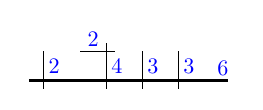
\begin{tikzpicture}[xscale=0.57,yscale=0.62]
\draw[thick,shorten >=2] (-1/3,0)--(127/30,0) node[inner sep=2pt,blue,above left,scale=0.8] {6};
\draw[shorten <=-3pt] (0,0)--node[inner sep=2pt,scale=0.8,blue,right] {2} (0,3/5);
\draw[shorten <=-3pt, shorten >=-3pt] (7/5,0)--node[inner sep=2pt,scale=0.8,blue,right] {4} (7/5,3/5);
\draw[shorten <=-3pt] (7/5,3/5)--node[inner sep=2pt,scale=0.8,blue,above] {2} (4/5,3/5);
\draw[shorten <=-3pt] (11/5,0)--node[inner sep=2pt,scale=0.8,blue,right] {3} (11/5,3/5);
\draw[shorten <=-3pt] (3,0)--node[inner sep=2pt,scale=0.8,blue,right] {3} (3,3/5);
\end{tikzpicture}
\end{document}
